% SOD toolbox user manual.  Compile with XeLaTeX:  latexmk -xelatex SOD_manual.tex
\documentclass[report]{nld}
\usepackage{amsmath,amsthm}
\usepackage{array,tabularx,longtable}
\usepackage{listings}

\newtheorem{proposition}{Proposition}

\newcommand{\X}{\mathbf{X}}
\newcommand{\V}{\mathbf{V}}
\newcommand{\Y}{\mathbf{Y}}
\newcommand{\Q}{\mathbf{Q}}
\newcommand{\M}{\mathbf{M}}
\newcommand{\K}{\mathbf{K}}
\newcommand{\Lm}{\mathbf{L}}
\newcommand{\G}{\mathbf{G}}
\newcommand{\x}{\mathbf{x}}
\newcommand{\y}{\mathbf{y}}
\newcommand{\q}{\mathbf{q}}
\newcommand{\Sg}{\symbf{\Sigma}}
\newcommand{\Ps}{\symbf{\Psi}}
\newcommand{\Ph}{\symbf{\Phi}}
\newcommand{\psib}{\symbf{\psi}}
\newcommand{\phib}{\symbf{\phi}}
\newcommand{\etab}{\symbf{\eta}}
\newcommand{\avg}[1]{\langle #1\rangle}
\newcommand{\code}[1]{\texttt{#1}}
\setlength{\emergencystretch}{3em}

\definecolor{codebg}{HTML}{F1EFE9}
\lstdefinestyle{nld}{basicstyle=\ttfamily\footnotesize, breaklines=true, backgroundcolor=\color{codebg},
  frame=single, rulecolor=\color{nldhairline}, framesep=5pt, xleftmargin=6pt, xrightmargin=6pt,
  keywordstyle=\color{nldnavy}\bfseries, commentstyle=\color{nldmuted}, stringstyle=\color{nldcopperdeep},
  columns=fullflexible, keepspaces=true, showstringspaces=false, upquote=true, aboveskip=0.8em, belowskip=0.8em}
\lstset{style=nld}

\title{SOD toolbox}
\subtitle{User manual for smooth orthogonal decomposition\\ in Python and MATLAB, version 0.3}
\reportnumber{User manual}
\author{Nonlinear Dynamics Laboratory}
\date{October 2026}
\runninghead{SOD toolbox \textperiodcentered{} user manual \textperiodcentered{} github.com/nld-uri/sod-toolbox}

\begin{document}
\maketitle
\setcounter{tocdepth}{2}
{\small\tableofcontents}
\newpage

% =====================================================================
\section{Overview}

Smooth orthogonal decomposition (SOD) finds the coordinates of a multichannel
record that change most slowly in time. For a record $\X$ with $m$ samples (rows)
and $n$ channels (columns), and its time derivative $\V$, it solves one real
symmetric generalized eigenproblem,
\begin{equation}
  \Sg_v\,\psib=\mu\,\Sg_x\,\psib,\qquad \Sg_x=\avg{\x\x^\top},\quad \Sg_v=\avg{\dot\x\dot\x^\top},
  \label{eq:sod}
\end{equation}
with the values $\mu_i$ in ascending order. The covectors $\psib_i$ define the
smooth coordinates $\q=\X\Ps$; the smooth modes are $\Ph=\Sg_x\Ps$. SOD here is the temporal form: it smooths the coordinates in time. Its spatial dual, smooth mode decomposition (SMD)~\cite{Li2023}, smooths the mode shapes in space and suits full-field data that are richer in space than in time; Section~\ref{sec:smd} describes its implementation here. A smooth mode of SOD is the shape paired with a temporally smooth coordinate, not a spatially smoothed shape. The method
was introduced for vibration mode identification by Chelidze and
Zhou~\cite{Chelidze2006} and for randomly excited systems by Farooq and
Feeny~\cite{Farooq2008}. The pencil itself, with first differences, appeared earlier in statistics as
maximum autocorrelation factors, for spatial imagery~\cite{Green1988} and for trends in parallel time series~\cite{Shapiro1989}.

For an undamped linear structure whose modal coordinates are uncorrelated over
the record, $\mu_i=\omega_i^2$ and the smooth modes are the linear normal modes
(LNMs). The smooth orthogonal values (SOVs) $\lambda_i=1/\mu_i$ are then the
reciprocal squared natural frequencies. Everything else in this toolbox is
either this pencil formed in a different way, or a rule for reading its output.

\paragraph{What the toolbox provides.}
\begin{itemize}
  \item \textbf{One canonical pencil} with the options that the SOD papers use:
    derivative estimate, step size, lagged covariances, centring, channel scaling
    and data-rank restriction (Section~\ref{sec:decomposition}).
  \item \textbf{State SOD} on $\y=(\x,\dot\x)$, which returns each damped mode as a
    pair of coordinates spanning its modal plane (Section~\ref{sec:damping}).
  \item \textbf{Recognition rules.} Modes are kept by spectral consistency and
    planes are paired by circularity, never by the SOD value (Section~\ref{sec:recog}).
  \item \textbf{Damping} from a free decay: plane-wise and subspace fits, and an
    identity that ties the damping estimate to the end states of the record.
  \item \textbf{Windowed SOD} for slowly varying records, such as the decay of a
    nonlinear mode (Section~\ref{sec:nonlinear}).
  \item \textbf{Reduced-order models}: LNM, MTA, POD, SOD and complex-mode bases,
    Galerkin and energy-Galerkin ROMs, exact simulation, and a
    linear-core-plus-residual basis for nonlinear structures.
\end{itemize}

\paragraph{Where to get it.} Code, manual, slides and animations:
\href{https://github.com/nld-uri/sod-toolbox}{\code{github.com/nld-uri/sod-toolbox}} (MIT license).

\paragraph{Contents of the toolbox.}
\begin{center}\small
\begin{tabularx}{\linewidth}{@{}>{\raggedright}p{4.3cm}X@{}}
\toprule
Folder & Contents\\
\midrule
\code{python/sodtoolbox/} & Python package (NumPy, SciPy; Matplotlib for figures)\\
\code{python/examples/} & ten worked examples (four SOD, six SMD) with their printed output\\
\code{python/tests/} & 15 self-contained tests; generator of the MATLAB reference data\\
\code{matlab/} & \code{sod\_*.m} functions in base MATLAB, no toolboxes\\
\code{matlab/examples/}, \code{test\_sod.m} & the same examples; 32 checks against Python\\
\code{docs/} & this manual, the slide deck and the animations\\
\bottomrule
\end{tabularx}
\end{center}

\subsection{Quick start}

Python:
\begin{lstlisting}[language=Python]
import numpy as np
import sodtoolbox as st                          # add python/ to sys.path
from sodtoolbox import systems as sy

M, K, C = sy.chain(4)                            # undamped 4-DOF chain
y0 = sy.equal_energy(M, K)                       # equal energy in every mode
t, X, V, A = sy.free_decay(M, K, C, y0, dt=0.02, N=200000)

R = st.sod(X, V)                                 # Sigma_v psi = mu Sigma_x psi
R.sov, R.freq, R.Phi, R.Q                        # 1/mu, sqrt(mu), smooth modes, coordinates
R2 = st.sod(X, dt=0.02)                          # velocities by central differences
\end{lstlisting}
MATLAB:
\begin{lstlisting}[language=Matlab]
addpath('path/to/sod-toolbox/matlab')
[M, K, C] = sod_chain(4);
y0 = sod_equal_energy(M, K);
[t, X, V, A] = sod_free_decay(M, K, C, y0, 0.02, 200000);
R  = sod_decomp(X, V);                           % R.mu, R.freq, R.sov, R.Psi, R.Phi, R.Q
R2 = sod_decomp(X, [], struct('dt', 0.02));
\end{lstlisting}

\paragraph{Choosing options.}
\begin{center}\small
\begin{tabularx}{\linewidth}{@{}>{\raggedright}p{5.4cm}X@{}}
\toprule
Your data & Use\\
\midrule
Displacement and velocity, exact or estimated & \code{sod(X, V)}\\
Displacement only, clean & \code{sod(X, dt=dt)}, then \code{cd\_correct} (Sec.~\ref{sec:fd})\\
Displacement with white sensor noise & \code{sod(X, dt=dt, h=2, lag=5)} or a regularised velocity (Sec.~\ref{sec:noise})\\
Channels in different units & \code{scale=True} (rank test only; Sec.~\ref{sec:rank})\\
Damped free decay; damping wanted & \code{state\_sod}, \code{pair\_state}, \code{decay\_damping} (Sec.~\ref{sec:damping})\\
Smooth trend under fast content & \code{sod(X, dt=dt, h=15, lag=31, center=True)} (Sec.~\ref{sec:trend})\\
Nonlinear free decay & \code{sod\_track(X, dt, nwin, step, boundary=True)}\\
Reduced-order model & \code{sod\_modes}, then \code{rom\_config} or \code{rom\_state} (Sec.~\ref{sec:rom})\\
\bottomrule
\end{tabularx}
\end{center}

% =====================================================================
\section{The decomposition}\label{sec:decomposition}

\subsection{Data and conventions}

Rows of $\X$ and $\V$ are time samples, columns are channels. Averages
$\avg{\cdot}$ are sample means. The toolbox normalises the covectors so that
$\psib_i^\top\Sg_x\psib_j=\delta_{ij}$. Then:
\begin{center}\small
\begin{tabular}{@{}ll@{}}
\toprule
Quantity & Definition\\
\midrule
smooth coordinates & $\q=\X\Ps$, unit variance\\
smooth modes & $\Ph=\Sg_x\Ps$, so $\Ps^\top\Ph=\mathbf{I}$ and $\X=\q\Ph^\top$ on the data subspace\\
SOD values & $\mu_i=\avg{\dot q_i^2}/\avg{q_i^2}$, the mean-square frequency of $q_i$\\
SOD frequencies & $\sqrt{\mu_i}$\\
smooth orthogonal values & $\lambda_i=1/\mu_i$\\
\bottomrule
\end{tabular}
\end{center}
By Parseval, $\mu_i$ is the power-weighted mean of $\omega^2$ over the spectrum of
$q_i$. For a Gaussian signal $\sqrt{\mu_i}/2\pi$ is the zero up-crossing
rate~\cite{Rice1944}.

\paragraph{Data-rank restriction.} When the record does not excite every
direction, $\Sg_x$ is singular. With \code{tol} set (default $10^{-10}$), the
pencil is solved on the eigenvectors of $\X^\top\X$ whose eigenvalues exceed
\code{tol} times the largest. The returned $\Ps$ and $\Ph$ are mapped back to all
channels.

\subsection{Geometry}\label{sec:geometry}

Each covector $\psib$ defines a scalar coordinate $q=\x^\top\psib$. The ratio
\begin{equation}
  \rho(\psib)=\frac{\psib^\top\Sg_v\psib}{\psib^\top\Sg_x\psib}=\frac{\avg{\dot q^2}}{\avg{q^2}}
\end{equation}
measures how rough $q$ is. SOD minimises $\rho$; the stationary values of $\rho$
are the $\mu_i$. POD, in contrast, maximises $\avg{q^2}$ alone and returns
orthogonal axes. The smooth modes are orthogonal only in the $\Sg_x^{-1}$ metric.

Figure~\ref{fig:geom} shows a two-mass chain with masses $(1,3)$ and springs
$(1,2)$. Its LNMs meet at $67.9^\circ$. The second POD axis is $24.6^\circ$ from the
second LNM; the second smooth mode is $0.002^\circ$ from it. The extremes of $\rho$
are $0.4381$ and $1.8643$, against $\omega=0.4380,\ 1.8641$
(\code{docs/animations/report\_numbers.py}).

\begin{figure}[h]
  \centering
  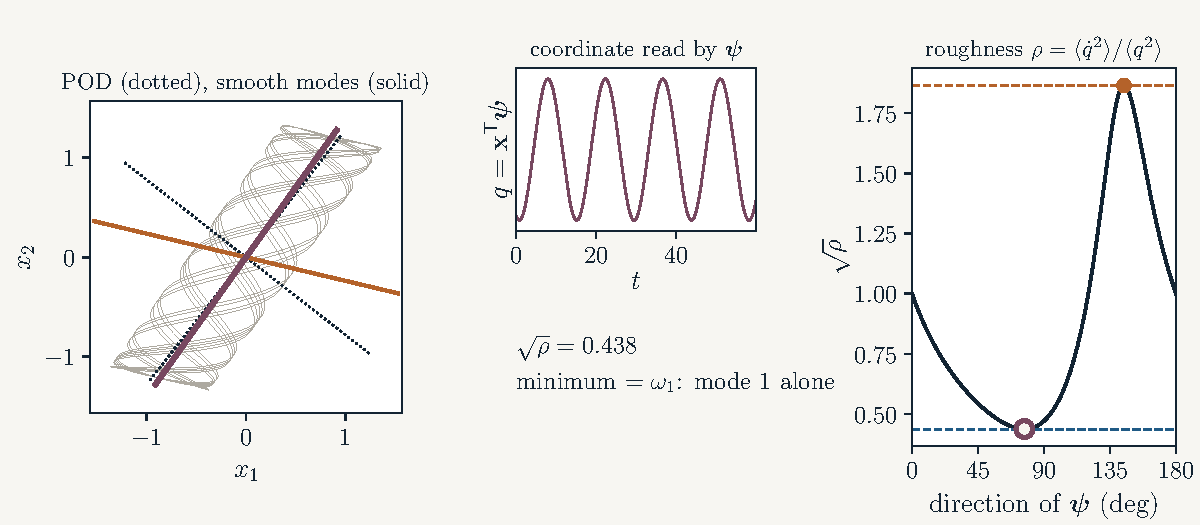
\includegraphics[width=\linewidth]{../animations/rayleigh_quotient_still.pdf}
  \caption{The roughness quotient of a two-mass chain. Left: displacement cloud,
  POD axes (dotted), smooth modes (blue, copper) and the direction read by a trial
  covector (plum). Middle: the coordinate it reads. Right: $\sqrt{\rho}$ against the covector direction; its
  extremes are $\omega_1$ and $\omega_2$. Animation:
  \code{docs/animations/rayleigh\_quotient.mp4}.}
  \label{fig:geom}
\end{figure}

\subsection{When is SOD exact?}\label{sec:exact}

Let $\Ph_0$ be the mass-normalised LNMs and $\etab=\Ph_0^{-1}\x$ the modal
coordinates, with modal covariances $\G_x=\avg{\etab\etab^\top}$ and
$\G_v=\avg{\dot{\etab}\dot{\etab}^\top}$.

\begin{proposition}[Exactness]\label{prop:exact}
SOD returns $\Ps=\Ph_0^{-\top}$ and $\mu_i=\omega_i^2$, up to scaling and order, if
(i) $\G_x$ and $\G_v$ are both diagonal (modal decorrelation) and (ii)
$(\G_v)_{ii}=\omega_i^2(\G_x)_{ii}$ for each mode (modal virial balance). For
distinct values the conditions are also necessary.
\end{proposition}

Every SOD bias violates (i), (ii) or both. Write
$\delta_i=(\G_v)_{ii}/(\omega_i^2(\G_x)_{ii})-1$ for the virial defect. To first
order the frequency bias is $\delta_i/2$, and modal correlation enters at second
order. On a finite undamped record both conditions hold only approximately, so
the bias is set by the record, not by the method.

\paragraph{Example 1.} \code{ex01\_linear\_chain} uses a 4-DOF chain with equal
modal energies and exact velocities. Over $T=4000$ time units,
$\lambda_i\omega_i^2-1$ was $5.2\times10^{-4}$, $3.1\times10^{-4}$,
$-8.9\times10^{-5}$ and $5.0\times10^{-5}$. The smooth modes matched the LNMs with
MAC $\ge0.99999994$. The error did not fall monotonically with record length
($T=250$, 1000 and 4000 gave $1.2$, $2.5$ and $0.5\times10^{-3}$ at most); it
follows the residual modal correlation of each record.

\begin{figure}[h]
  \centering
  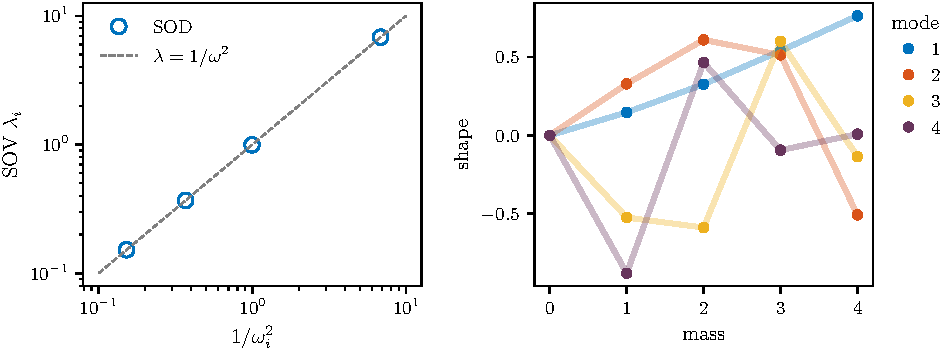
\includegraphics[width=\linewidth]{figures/ex01_linear_chain.pdf}
  \caption{Example 1. Left: SOVs against $1/\omega_i^2$. Right: smooth modes (dots)
  and LNMs (lines).}
  \label{fig:ex01}
\end{figure}

\subsection{What damping does}\label{sec:dampingtheory}

Damping breaks the correspondence in two ways, depending on the record.

\paragraph{Stationary response.} With forcing and damping, the exact covariance
identity reads $\Sg_x^{-1}\Sg_v=\mathbf{A}^\top+\Sg_x^{-1}\mathbf{S}\mathbf{B}^\top$, where
$\mathbf{S}$ is the skew part of $\avg{\x\dot\x^\top}$ (the circulation). SOD never forms
$\mathbf{S}$, so this term biases it. If the forcing covariance is proportional to
the damping matrix, $\mathbf{S}=\mathbf{0}$ and SOD is exact for any damping. The bias
comes from the mismatch between forcing and damping, not from the damping class
(Bellizzi and Sampaio~\cite{Bellizzi2009} reported exactness for uncorrelated modal
forcing).

\paragraph{Free decay.} Integration by parts leaves a boundary term, the energy
lost over the record. Take a single-DOF decay with $\eta(0)=a\cos\varphi$ and
$\dot\eta(0)=-\omega a\sin\varphi$, recorded until it has died out. Its SOD value is
\begin{equation}
  \mu=\frac{\omega^2}{1+4\zeta^2\cos^2\varphi-2\zeta\sin2\varphi}.
\end{equation}
Released from rest ($\varphi=0$) the defect is $-4\zeta^2/(1+4\zeta^2)$, second order
in $\zeta$; an initial velocity adds a first-order term that averages to zero over
$\varphi$. In a multi-mode decay the modes also stay correlated,
because the record lasts only about $1/\zeta\omega$. Example~4 shows
configuration-SOD frequency errors of $0.2$--$1.5\%$ at $\zeta\approx1.3$--$2\%$.

\paragraph{State SOD.} Apply the same pencil to the state $\y=(\x,\dot\x)$:
\begin{equation}
  \avg{\dot\y\dot\y^\top}\psib=\mu\avg{\y\y^\top}\psib .
\end{equation}
The pencil stays real and symmetric and is invariant under any change of state
coordinates. Each complex mode $s_i=\sigma_i+\mathrm{i}\,\omega_{d,i}$ owns a real
plane on which $\dot{\symbf\xi}_i=\Lm_i\symbf\xi_i$.

\begin{proposition}[State SOD]\label{prop:ssod}
If the modal planes are uncorrelated, the values split by plane and the two values
of plane $i$ satisfy $\mu_{i,a}\mu_{i,b}=|s_i|^4$. The two smooth modes of the pair
span the modal plane. The two values are equal if and only if the plane covariance
is isotropic.
\end{proposition}

So the geometric mean of a pair returns $|s_i|$ for any damping, without the
virial balance. The plane itself carries the damping: a least-squares fit
$\Lm=\avg{\dot\q\q^\top}\avg{\q\q^\top}^{-1}$ on the two coordinates gives
$s_i$ and $\zeta_i=-\tfrac12\mathrm{tr}\,\Lm/\sqrt{\det\Lm}$ (Section~\ref{sec:damping}).

% =====================================================================
\section{Practical data}\label{sec:practical}

\subsection{Velocities from displacement}\label{sec:fd}

\code{sod(X, dt=dt)} forms $\V$ by central differences,
$v_j=(x_{j+h}-x_{j-h})/2h\Delta t$, and drops $h$ samples at each end;
\code{deriv='gradient'} keeps every sample. A central difference multiplies a
sinusoid of frequency $\omega$ by $\sin(\omega h\Delta t)/(\omega h\Delta t)$, so an
exact mode returns $\sin(\omega h\Delta t)/h\Delta t$. The relative error is about
$-(\omega h\Delta t)^2/6$. \code{cd\_correct(w, h*dt)} inverts it.

\paragraph{Example 2.} On the chain of Example~1, at $\Delta t=0.4$ the raw error of
mode~4 ($\omega\Delta t=1.02$) was $-0.17$. After \code{cd\_correct} every error fell
to the finite-record floor of Example~1, below $2.6\times10^{-4}$ in frequency.

\begin{figure}[h]
  \centering
  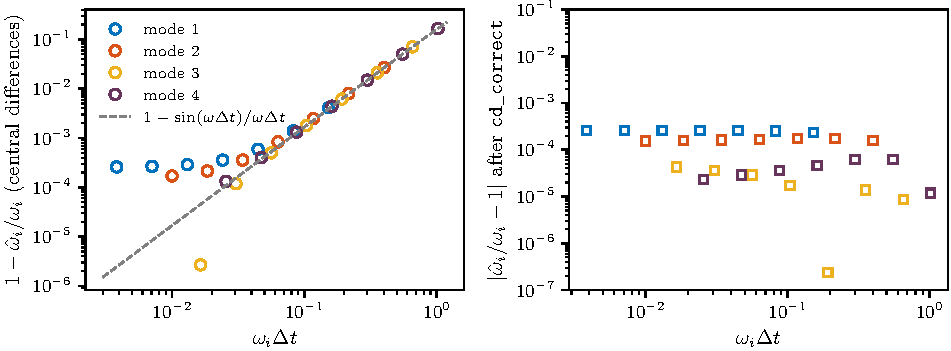
\includegraphics[width=\linewidth]{figures/ex02_fd_bias.pdf}
  \caption{Example 2. Left: central-difference error against $\omega\Delta t$ and
  the prediction $1-\sin(\omega\Delta t)/\omega\Delta t$. Right: the error after
  \code{cd\_correct}.}
  \label{fig:ex02}
\end{figure}

\subsection{Sensor noise}\label{sec:noise}

A central difference turns white sensor noise into roughness. Every SOD frequency
rises, and fast noise directions can take the place of weak modes. Two remedies are
built in.
\begin{itemize}
  \item \textbf{Lagged covariances.} \code{lag=$\ell$} replaces both covariances by the
    symmetrised lag-$\ell$ covariances. With $\ell\ge2h+1$ white noise drops out of
    both. The pencil stays real and symmetric but may become indefinite in fast
    directions; those values sort last.
  \item \textbf{Regularised velocities.} Estimate $\V$ with a smoother (for example the
    lab's kinematics toolbox) and call \code{sod(X, V)}.
\end{itemize}

\paragraph{Example 3.} A 6-DOF chain ($\zeta=2\%$) was driven at its last mass by
noise band-limited at $2.6$~rad/s, between modes 5 and 6, and the displacements
carried 1\% white sensor noise. With central differences the six SOD frequencies
were $0.282$, $0.788$, $1.385$, $3.627$, $14.28$ and $15.76$~rad/s, and recognition kept
only the first coordinate. With $h=2$ and lag~5 they were $0.271$, $0.739$, $1.167$,
$1.564$, $1.849$ and $8.43$; recognition kept modes 1--4, at peaks $0.270$, $0.735$,
$1.168$ and $1.566$ (true $0.271$, $0.741$, $1.174$, $1.582$). Mode~5, weakly excited
near the cutoff, mixed with noise and was rejected.

\begin{figure}[h]
  \centering
  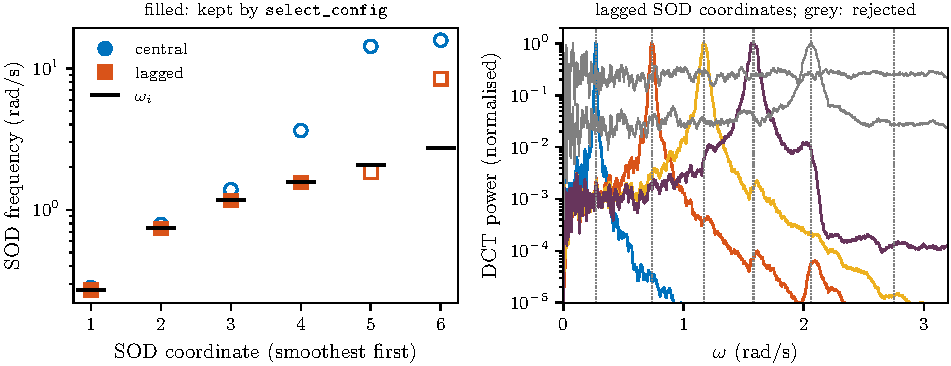
\includegraphics[width=\linewidth]{figures/ex03_noise_recognition.pdf}
  \caption{Example 3. Left: SOD frequencies with central differences and with lagged
  covariances; filled markers were kept by \code{select\_config}. Right: DCT spectra
  of the lagged-SOD coordinates; grey: rejected.}
  \label{fig:ex03}
\end{figure}

\subsection{Rank and channel scaling}\label{sec:rank}

The pencil is invariant to channel scaling for full-rank data. The rank cut is not.
\code{scale=True} divides each channel by its RMS before the rank test and maps the
result back to the original units. On a forced cantilever record of data rank 9 out
of 60, scaled and unscaled SOD kept different weak directions and agreed only on the
two smoothest values. Use \code{scale=True} when channels carry different units,
as in state SOD.

\subsection{Recognising modes}\label{sec:recog}

The smoothness order is not the mode order. A noise direction, a drift or a mixed
coordinate can be smoother than a weakly excited mode. The toolbox therefore never
selects or pairs coordinates by $\mu_i$.
\begin{itemize}
  \item \code{select\_config}: keep coordinate $i$ if the peak of its smoothed DCT-II
    periodogram lies within $\max(5\%,\ \text{half-power width})$ of $\sqrt{\mu_i}$ and
    below a frequency limit. The width is capped at 15\%, so a drifting coordinate,
    whose spectrum peaks near zero, cannot pass. Coordinates sharing one peak keep
    only the one with the largest response energy.
  \item \code{pair\_state}: pair two state-SOD coordinates if their peaks agree and the
    spectrum of $q_a+\mathrm{i}q_b$ is one-sided by at least 0.85. A pair between 0.75
    and 0.85 is rescued if its banded one-sidedness is at least 0.95 and it carries at
    least 1\% of the response energy.
\end{itemize}

\subsection{Smooth trends}\label{sec:trend}

SOD needs no dynamics. Any record whose sources are uncorrelated over the record,
with uncorrelated derivatives, is unmixed exactly. With \code{center=True}, a
step $h$ and a lag, the smoothest coordinate is a trend estimate. In
Figure~\ref{fig:trend}, six channels mix a half-cycle drift, a slow cycle and four
fast sources. With $h=15$ and lag~31 the drift error at 0.3, 1 and 3\% sensor noise
was $7.9\times10^{-3}$, $2.6\times10^{-2}$ and $8.1\times10^{-2}$. The oracle unmixing
$\mathbf{A}^{-1}$ gave $7.8\times10^{-3}$, $2.6\times10^{-2}$ and $7.8\times10^{-2}$. The
leading POD coordinate correlated with the drift at $0.010$.

\begin{figure}[h]
  \centering
  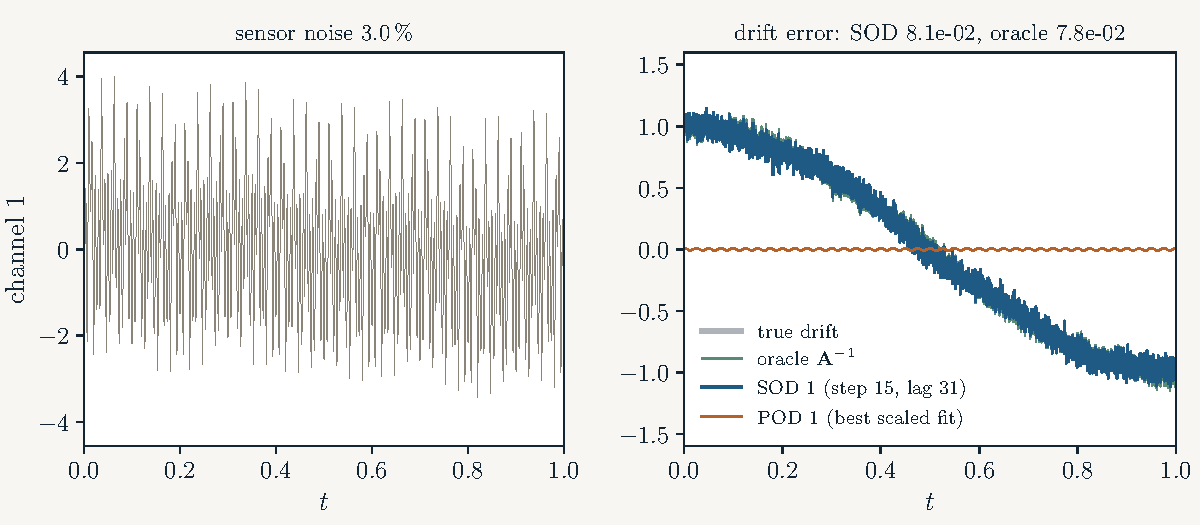
\includegraphics[width=\linewidth]{../animations/trend_extraction_still.pdf}
  \caption{Trend extraction at 3\% sensor noise. Left: one observed channel. Right:
  the true drift, the smoothest SOD coordinate, the oracle unmixing and the best scaled
  fit of the leading POD coordinate. Animation:
  \code{docs/animations/trend\_extraction.mp4}.}
  \label{fig:trend}
\end{figure}

% =====================================================================
\section{Damping from a free decay}\label{sec:damping}

\code{decay\_damping(R, Yd, dt, wmax)} takes a state-SOD result and the state
derivative. For each plane found by \code{pair\_state} it fits
$\Lm=\avg{\dot\q\q^\top}\avg{\q\q^\top}^{-1}$ and returns $s$ and $\zeta$. It also fits
$\Lm$ on the $k$ smoothest coordinates at once (the subspace fit, a
continuous-time least-squares relative of DMD~\cite{Schmid2010}) and returns its
eigenvalues.

\paragraph{The damping identity.} For free response the trace of a plane fit
depends only on the end states,
\begin{equation}
  \mathrm{tr}\,\Lm=\frac{\q_T^\top\G^{-1}\q_T-\q_0^\top\G^{-1}\q_0}{2T},\qquad \G=\avg{\q\q^\top}.
\end{equation}
So the estimate needs a record that has decayed, or a known end state. The identity
is exact for the chord derivative $(q_{k+1}-q_k)/\Delta t$. With exact $\dot q$ and
sampled sums the two forms differ by a relative $O((|s|\Delta t)^2/\zeta)$, because
the integrand oscillates with size $|s|$ about a mean $\zeta|s|$.

\paragraph{Example 4.} A 4-DOF chain with Rayleigh damping (2\% at modes 1 and 4)
decayed from equal modal energies. Configuration SOD erred in frequency by
$+0.21$, $-0.82$, $+1.5$ and $-1.3\%$. State SOD gave four planes with circularity
$0.992$--$0.995$. The per-plane damping erred by $3.6\times10^{-4}$, $-2.7\times10^{-4}$,
$-5.2\times10^{-3}$ and $8.6\times10^{-3}$ (relative); a tilted plane leaks the dynamics
of its neighbour. The subspace fit returned every $\zeta$ to $2.4\times10^{-14}$ or better.

\begin{figure}[h]
  \centering
  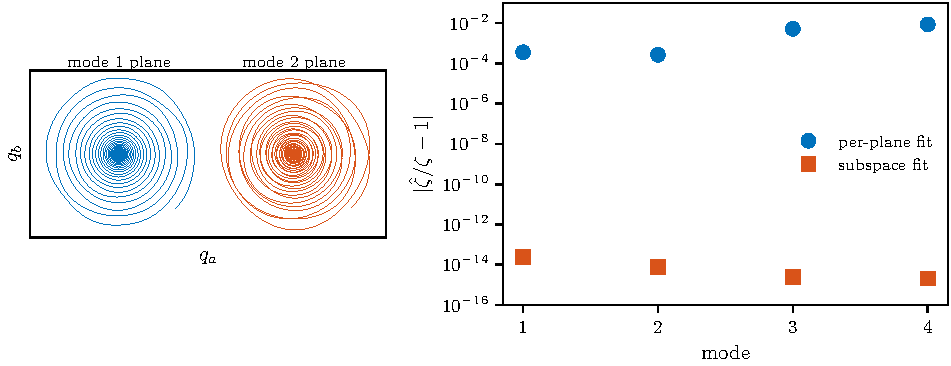
\includegraphics[width=\linewidth]{figures/ex04_damped_decay.pdf}
  \caption{Example 4. Left: the coordinate pairs of the mode~1 and mode~2 planes.
  Right: relative damping error of the per-plane and subspace fits.}
  \label{fig:ex04}
\end{figure}

\begin{figure}[h]
  \centering
  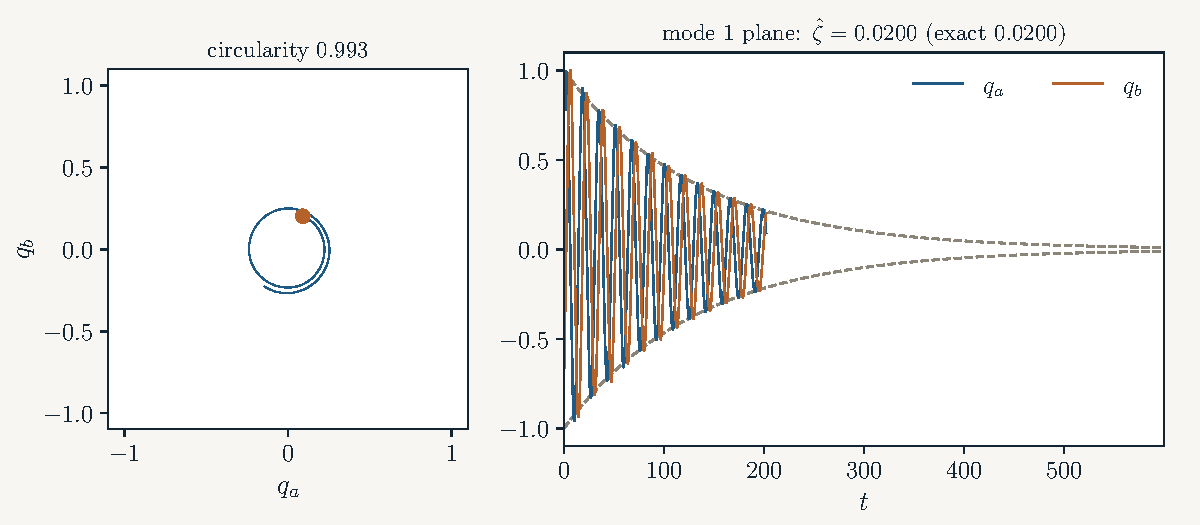
\includegraphics[width=\linewidth]{../animations/state_plane_still.pdf}
  \caption{The mode~1 plane of Example~4 as it decays. Animation:
  \code{docs/animations/state\_plane.mp4}.}
  \label{fig:plane}
\end{figure}

% =====================================================================
\section{Nonlinear systems and reduced-order models}\label{sec:nonlinear}

\subsection{Windowed SOD}

\code{sod\_track(X, dt, nwin, step, boundary)} slides a window of \code{nwin}
samples along the record and returns, per window, the frequency and smooth mode of
the smoothest coordinate. Velocities are central differences inside the window.
\code{boundary=True} subtracts the symmetric part of the boundary term
$(\x_T\dot\x_T^\top-\x_0\dot\x_0^\top)/T$ from $\Sg_v$, which removes the leading
finite-window bias for undamped motion.

Figure~\ref{fig:backbone} follows a hardening two-mass chain (cubic spring at mass~1,
$\zeta=0.5\%$) from an amplitude where mode~1 is 12\% stiffer than linear. Against the
zero-crossing frequency of $x_1$, windows of 12 linear periods deviated by a median
$4.1\times10^{-4}$ with the boundary correction and $3.2\times10^{-3}$ without; the
largest deviation was about 3\% in both. Windowed values are equivalent-linear values
of the window. The SOD frequency is a mean-square frequency, so higher harmonics of
the orbit raise it.

\begin{figure}[h]
  \centering
  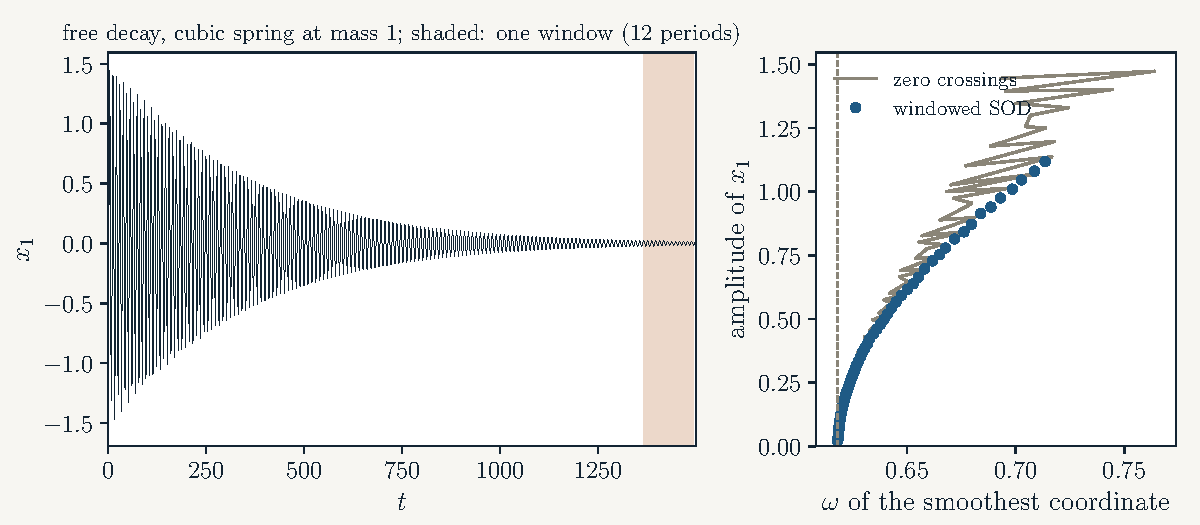
\includegraphics[width=\linewidth]{../animations/backbone_tracking_still.pdf}
  \caption{Windowed SOD along a hardening decay. Left: the record and one window.
  Right: frequency of the smoothest coordinate against window amplitude, and the
  zero-crossing frequency. Animation: \code{docs/animations/backbone\_tracking.mp4}.}
  \label{fig:backbone}
\end{figure}

\subsection{Reduced-order models}\label{sec:rom}

\begin{itemize}
  \item \textbf{Bases.} \code{lnm}, \code{mta} (LNMs plus static load vectors,
    $\M$-orthonormal), \code{pod}, \code{sod\_modes} (unit-norm smooth modes on the
    data subspace) and \code{complex\_modes} (slowest eigen-planes in real form).
  \item \textbf{Configuration ROM.} \code{rom\_config} projects $\M,\K,\mathbf{C}$ and
    the load map on a basis and simulates exactly under zero-order-hold input.
  \item \textbf{State ROM.} \code{rom\_state(..., W=energy\_weight(M, K))} is an
    energy-Galerkin projection on the smooth modes of state SOD. Petrov--Galerkin with
    the data covectors (\code{W=None}) is not stable in general and is kept only for
    comparison.
  \item \textbf{Linear core plus residual.} For nonlinear data, \code{residual\_basis}
    fits $\ddot\q\approx\K_a\q+\mathbf{C}_a\dot\q$ on the $r_1$ smoothest SOD coordinates
    and adds the leading directions of the equation error. The useful variant is
    \code{kind='k'}: the quasi-static displacement $\K^{-1}\M\mathbf{e}$ driven by the
    residual force. The acceleration-level residual (\code{'a'}) and its low-passed
    form (\code{'f'}) were not useful in our nonlinear-beam tests.
\end{itemize}

% =====================================================================
\section{Smooth mode decomposition}\label{sec:smd}
SMD exchanges the roles of space and time~\cite{Li2023}. With snapshots $\symbf W$ (snapshots $\times$ points),
quadrature weights $\symbf w$ and spatial derivative fields $\symbf G_k$ of the same snapshots,
\begin{equation}
\symbf S_G\symbf p=\mu\,\symbf S_W\symbf p,\qquad \symbf S_W=\symbf W\,\mathrm{diag}(\symbf w)\,\symbf W^\top,\quad
\symbf S_G=\textstyle\sum_k c_k\,\symbf G_k\,\mathrm{diag}(\symbf w)\,\symbf G_k^\top .
\end{equation}
Each covector $\symbf p$ gives a mode $\symbf{\phi}=\symbf W^\top\symbf p$ of unit weighted norm, and
$\mu=\|D\symbf{\phi}\|^2/\|\symbf{\phi}\|^2$ is the Rayleigh quotient of the spatial operator $D$.
For a sinusoidal shape $\mu=k^{2m}$, with $m$ the operator order; $k=\mu^{1/(2m)}$ is the SMD wavenumber.
\begin{itemize}
\item Operators: \code{'grad'} ($m=1$; strings, membranes, flows), \code{'second'} ($m=2$; beams, and the Hessian with weight 2 on the mixed term on grids), \code{'laplacian'} ($m=2$), \code{'plate'} ($m=2$; Kirchhoff bending energy $(1-\nu)(w_{xx}^2+2w_{xy}^2+w_{yy}^2)+\nu(\nabla^2w)^2$, Poisson ratio \code{nu}).
\item Physical weights: \code{density} (mass per length or area) multiplies the weights of $\symbf S_W$ and \code{stiffness} ($T$, $EI$ or the plate rigidity) those of $\symbf S_G$. For a self-adjoint structure matched by the operator, $\mu_i=\omega_i^2$ (\code{R.omega}) and the modes are mass-normalized, from any snapshots that span them. Unit weights bias the modes of non-uniform structures, which are mass-orthogonal, not $L^2$-orthogonal.
\item \code{maf} is the maximum autocorrelation factor transform (Switzer and Green, 1984) with snapshots as bands: SMD with a forward-difference gradient and unit weights (\code{axes='xy'}), or with a single directional difference (\code{axes='x'} or \code{'y'}, the single lag of Green et al., 1988).
\item Derivative estimators: \code{'fd'} (second-order finite differences, also on non-uniform lines; a derivative is kept only where its stencil is measured), \code{'whittaker'} (penalized smoothing with gain $1/(1+(k/k_c)^{2p})$; fills masked points), \code{'savgol'} (local polynomials on complete uniform grids; the window is set from the measured half-gain cutoff).
\item Both integrals run over the points where the derivative is valid. Snapshot order, spacing and rate are never used.
\item Cutoffs: in the beam test with 0.5\% noise, Whittaker needed $k_c$ about 3--6 times and Savitzky--Golay about 8 times the largest wavenumber of interest. Scan $k_c$ with \code{smd\_kc\_scan} and keep a value where the wavenumbers do not move.
\item Conditioning: the Whittaker system has condition number up to about $1+(2/(h k_c))^{2p}$; above $10^{12}$ a warning is issued.
\item Implementation: $\symbf S_W$ is never formed. The thin SVD of the weighted field gives the data span, and the pencil is solved on it, so long records (many snapshots) cost $O(n_t n r)$.
\end{itemize}
\paragraph{What the tests establish.} SMD values depend only on the span of the snapshots, so shuffled or
correlated snapshots give identical results. With the operator matched to the stiffness on a complete
domain, strings, cantilever beams and membranes return their modes and wavenumbers to discretization error.
A hole in the field, a partial field of view or a mismatched operator biases them. These are the spatial
counterparts of SOD's boundary terms. With physical weights a tapered pinned--pinned beam returns its
frequencies to $1.3\times10^{-4}$ from five snapshots (\code{python/tests/test\_smd.py}, 32 checks;
\code{matlab/test\_smd.m}, 43 checks including agreement with Python).

\subsection{SMD examples}\label{sec:smd-examples}
Examples 5--10 (\code{python/examples/ex05}--\code{ex10}, with MATLAB twins) store their printed output next to the scripts. Every number below is copied from those outputs.

\paragraph{Example 5: snapshots without time.} A fixed rectangular membrane ($a=1$, $b=0.7$, $81\times57$ grid) carries a random combination of its first eight modes. SMD with the gradient returns the modes ($1-\mathrm{MAC}\le6.7\times10^{-8}$) and the wavenumbers to $4.0\times10^{-3}$ from 200 snapshots, from the same snapshots shuffled, and from only eight. The remaining error is the central-difference bias, the spatial twin of Example~2.
\begin{figure}[h]
  \centering
  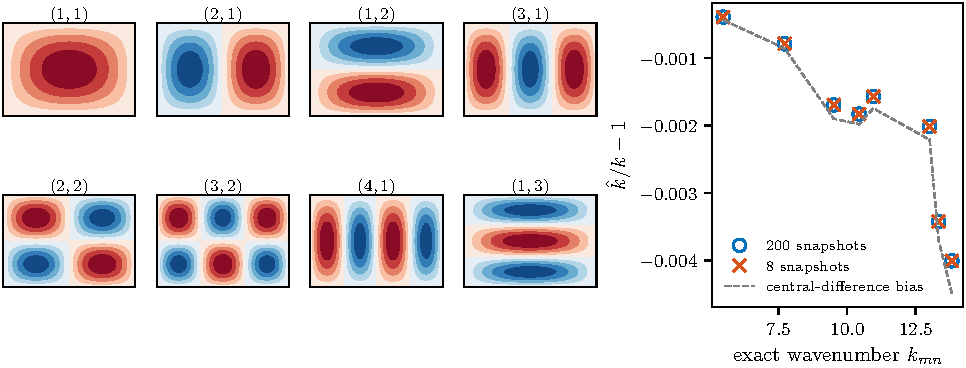
\includegraphics[width=1\linewidth]{figures/ex05_smd_membrane.pdf}
  \caption{Example 5. Left: the eight SMD modes. Right: wavenumber error from 200 and from 8 snapshots, against the central-difference prediction.}
  \label{fig:ex05}
\end{figure}

\paragraph{Example 6: physical weights.} A pinned--pinned beam with $EI=1$ and $\rho A=1+2x$. Its modes are mass-orthogonal, not $L^2$-orthogonal, so unit weights bias the shapes ($1-\mathrm{MAC}$ up to $0.15$). With \code{density} and \code{stiffness}, six snapshots give the modes to $1-\mathrm{MAC}\le2.1\times10^{-9}$ and the frequencies of a 100-term Galerkin model to $1.9\times10^{-4}$ on 401 points; the error falls as $h^2$.
\begin{figure}[h]
  \centering
  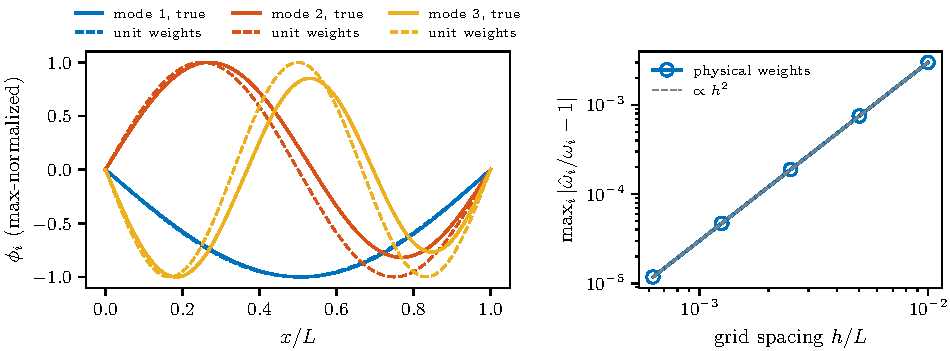
\includegraphics[width=1\linewidth]{figures/ex06_smd_nonuniform_beam.pdf}
  \caption{Example 6. Left: true modes (solid) and unit-weight SMD modes (dashed). Right: frequency error with physical weights against grid spacing.}
  \label{fig:ex06}
\end{figure}

\paragraph{Example 7: noise and the cutoff.} A cantilever (three modes, 40 snapshots) with 0.1, 0.5 and 2\% white noise, ten realizations each. Plain finite differences give wavenumber errors of 3.8, 9.5 and 20 (medians). Whittaker smoothing brings them to $8\times10^{-4}$, $2.8\times10^{-3}$ and $8.1\times10^{-3}$ at its best cutoff, which falls from about $5\,k_{\max}$ to $3\,k_{\max}$ as noise grows; Savitzky--Golay is 2.4--4.3 times worse.
\begin{figure}[h]
  \centering
  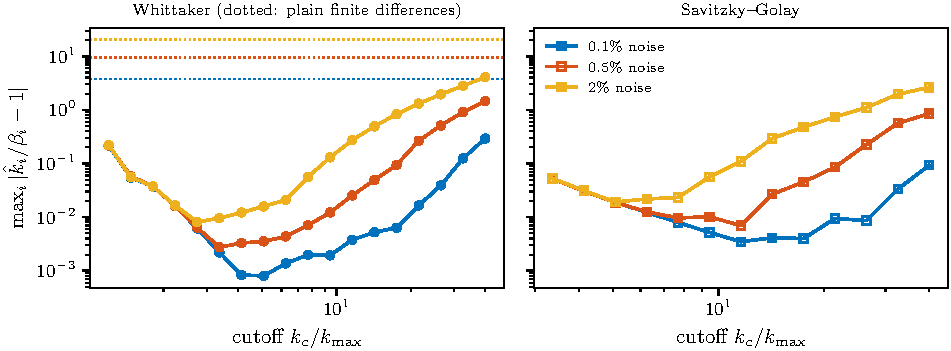
\includegraphics[width=1\linewidth]{figures/ex07_smd_noise.pdf}
  \caption{Example 7. Median wavenumber error against the cutoff for Whittaker (left; dotted: plain finite differences) and Savitzky--Golay (right).}
  \label{fig:ex07}
\end{figure}

\paragraph{Example 8: boundaries.} Exactness needs orthogonality over the measured domain. A centred field of view of $0.8L$ on a cantilever biases the wavenumbers by $-11.5$, $+1.8$ and $+11\%$. A circular hole of radius $0.14$ in a membrane biases the $(1,1)$ mode by $+11\%$. These are the spatial counterparts of SOD's window bias.
\begin{figure}[h]
  \centering
  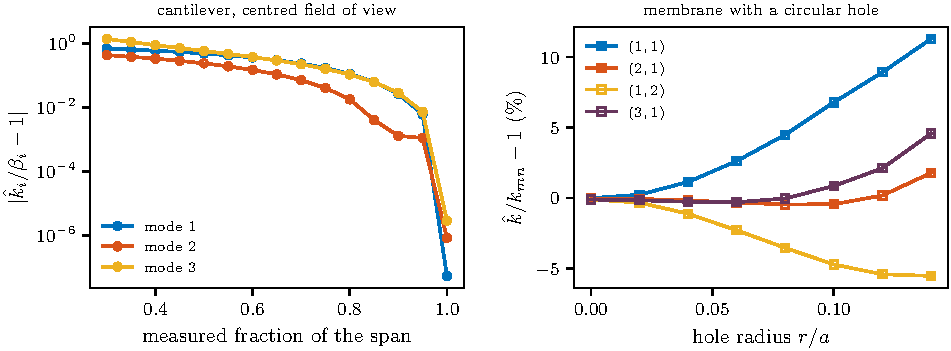
\includegraphics[width=1\linewidth]{figures/ex08_smd_boundaries.pdf}
  \caption{Example 8. Left: cantilever, wavenumber bias against the measured fraction of the span. Right: membrane, bias against hole radius.}
  \label{fig:ex08}
\end{figure}

\paragraph{Example 9: sub-Nyquist and random snapshots.} A simply supported beam ($\omega_j=(j\pi)^2$, highest mode at 56.5~Hz) decays freely for 10~s. SMD with physical weights gives all six frequencies to $1.85\times10^{-4}$ at every sampling rate from 400~Hz down to 2~Hz, and from 12 randomly timed snapshots. SOD with central differences fails once $\omega_6\Delta t$ is large (error $0.25$ at $f_s=3.5f_6$, near 1 below Nyquist). With exact velocities SOD often survives undersampling but fails erratically where aliased frequencies nearly coincide.
\begin{figure}[h]
  \centering
  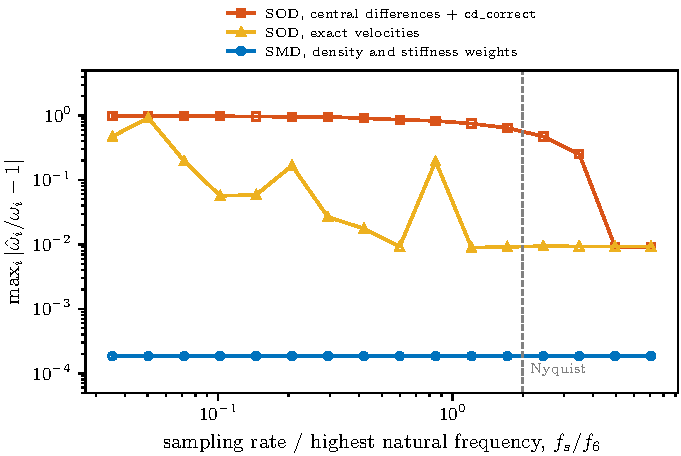
\includegraphics[width=0.75\linewidth]{figures/ex09_smd_subnyquist.pdf}
  \caption{Example 9. Largest frequency error against the sampling rate for SMD and SOD.}
  \label{fig:ex09}
\end{figure}

\paragraph{Example 10: a plate.} A simply supported plate ($a=1$, $b=0.6$, $D=\rho h=1$, $\nu=0.3$) has $\omega_{mn}=\pi^2[(m/a)^2+(n/b)^2]$. With physical weights the \code{plate} operator returns the first eight frequencies to within $0.21\%$; the Hessian and Laplacian operators agree with it to discretization error, because the Gaussian-curvature term vanishes on simply supported edges.
\begin{figure}[h]
  \centering
  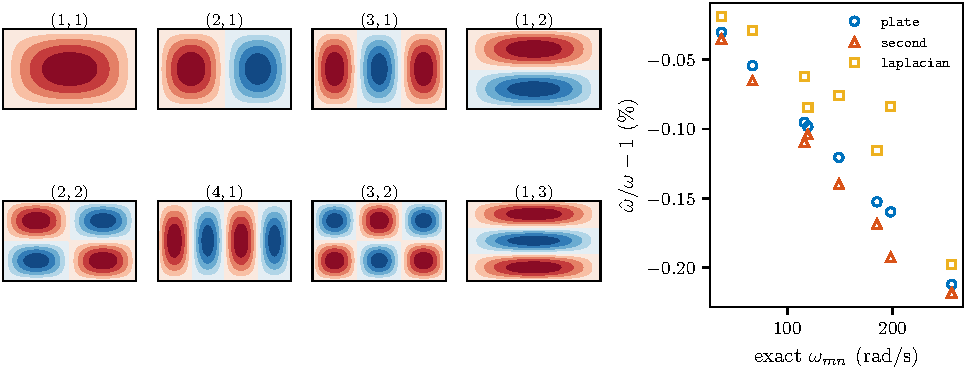
\includegraphics[width=1\linewidth]{figures/ex10_smd_plate.pdf}
  \caption{Example 10. Left: the eight SMD modes. Right: frequency error for the three operators.}
  \label{fig:ex10}
\end{figure}

\clearpage
\section{Reference}\label{sec:reference}

\subsection{Installation}
Python 3.10 or later with NumPy and SciPy (\code{pip install -r requirements.txt}).
Add \code{python/} to the path and \code{import sodtoolbox as st}. MATLAB R2020b or
later; add \code{matlab/} to the path. No MATLAB toolboxes are needed; the DCT is
computed from an FFT.

\subsection{Functions}
\begin{center}\small
\begin{longtable}{@{}>{\raggedright}p{4.6cm}>{\raggedright}p{4.0cm}p{6.2cm}@{}}
\toprule
Python (\code{sodtoolbox}) & MATLAB & Purpose\\
\midrule\endhead
\code{sod} & \code{sod\_decomp} & configuration SOD with all options\\
\code{state\_sod} & \code{sod\_state} & state SOD, unit-RMS rank test\\
\code{derivative} & \code{sod\_deriv} & central (step $h$) or gradient derivative\\
\code{data\_rank\_basis} & \code{sod\_rank\_basis} & basis of the data subspace\\
\code{covariances} & \code{sod\_cov} & plain or lagged symmetric covariances\\
\code{sod\_pencil} & \code{sod\_pencil} & pencil from given covariances\\
\code{boundary\_term}, \code{csod} & \code{sod\_boundary}, \code{sod\_csod} & boundary term; boundary-corrected fit\\
\code{sod\_window}, \code{sod\_track} & \code{sod\_window}, \code{sod\_track} & windowed SOD\\
\code{dct\_spectrum}, \code{peak\_and\_width} & \code{sod\_dct\_spectrum}, \code{sod\_peak\_width} & smoothed DCT periodogram, peak, width\\
\code{cd\_correct} & \code{sod\_cd\_correct} & invert the central-difference bias\\
\code{select\_config} & \code{sod\_select\_config} & mode recognition, configuration SOD\\
\code{pair\_state} & \code{sod\_pair\_state} & plane pairing, state SOD\\
\code{fit\_L}, \code{plane\_eigs}, \code{plane\_identity} & \code{sod\_fit\_L}, \code{sod\_plane\_eigs}, \code{sod\_plane\_identity} & plane fit, eigenvalue, damping identity\\
\code{decay\_damping} & -- & all damping estimates of a decay\\
\code{lnm}, \code{mta}, \code{pod}, \code{sod\_modes} & \code{sod\_lnm}, \code{sod\_mta}, \code{sod\_pod}, \code{sod\_modes} & reduction bases\\
\code{complex\_modes} & -- & complex-mode baseline\\
\code{galerkin}, \code{rom\_config}, \code{rom\_state} & \code{sod\_galerkin} & reduced matrices; simulated ROMs\\
\code{state\_matrices}, \code{zoh}, \code{simulate\_state} & -- & exact zero-order-hold simulation\\
\code{residual\_basis}, \code{residual\_diagnostics} & \code{sod\_residual\_basis} & linear core plus residual\\
\code{merr}, \code{mac}, \code{mortho}, \code{principal\_angles} & \code{sod\_merr}, \code{sod\_mac}, \code{sod\_mortho} & metrics\\
\code{systems.chain}, \code{systems.equal\_energy}, \code{systems.free\_decay} & \code{sod\_chain}, \code{sod\_equal\_energy}, \code{sod\_free\_decay} & benchmark chains\\
\code{systems.duffing\_decay} & -- & chain with a cubic spring\\
\code{plotting.set\_style} & \code{sod\_set\_style} & LaTeX text and palettes\\
\code{make\_grid} & \code{sod\_smd\_grid} & SMD grid, mask, quadrature weights\\
\code{smd\_derivatives} & \code{sod\_smd\_derivs} & spatial derivative fields\\
\code{smd}, \code{smd\_kc\_scan} & \code{sod\_smd}, \code{sod\_smd\_kc\_scan}, \code{sod\_smd\_mode} & smooth mode decomposition; cutoff scan\\
\code{maf} & \code{sod\_smd\_maf} & maximum autocorrelation factors\\
\bottomrule
\end{longtable}
\end{center}

\subsection{Options of \code{sod} / \code{sod\_decomp}}
\begin{center}\small
\begin{tabularx}{\linewidth}{@{}>{\raggedright}p{3.0cm}>{\raggedright}p{2.4cm}X@{}}
\toprule
Option & Default & Effect\\
\midrule
\code{V} & none & velocities; if absent, formed from \code{X} with \code{dt}\\
\code{deriv}, \code{h} & \code{'central'}, 1 & derivative estimate and step\\
\code{lag} & 0 & symmetric lag-\code{lag} covariances (general eigensolver)\\
\code{center} & false & remove the mean of \code{X} before differencing\\
\code{scale} & false & unit-RMS channels for the rank test; results in original units\\
\code{tol} & $10^{-10}$ & data-rank tolerance; \code{None} (\code{[]}) for no restriction\\
\code{k} & all & number of smoothest coordinates returned\\
\bottomrule
\end{tabularx}
\end{center}

\subsection{Result fields}
\code{mu} (ascending), \code{freq} ($\sqrt{\mu}$, NaN where $\mu\le0$), \code{sov}
($1/\mu$), \code{Psi} (covectors, $\psib^\top\Sg_x\psib=1$), \code{Phi} (smooth modes
$\Sg_x\Ps$), \code{Q} (coordinates for the samples used). Python also offers
\code{modes\_unit()}.

% =====================================================================
\section{Validation}

\begin{itemize}
  \item \code{python/tests/test\_sod.py}: 15 checks of known properties. They cover
    exact SOVs and covectors from exact covariances, the central-difference bias,
    recognition order, plane recognition and damping of a decay, the normal equations
    of the residual fit and the exact simulator. All pass.
  \item \code{matlab/test\_sod.m}: 32 checks of the MATLAB port against
    \code{sod\_reference.mat}, written by \code{make\_reference.py}. Agreement is
    $10^{-13}$ or better for the plain pencil and $10^{-9}$ for lagged and differenced
    variants; recognition returns the same coordinates. One circularity score differs by
    $1.3\times10^{-8}$ between the two FFT implementations.
  \item Before release, 28 checks compared the toolbox with the code that produced the
    SOD papers' results, and the papers' recognition, damping, mode-shape and nonlinear
    scripts were rerun on the toolbox without changing any printed number.
\end{itemize}

% =====================================================================
\section{Limitations}
\begin{itemize}
  \item SOD returns LNMs only under modal decorrelation and virial balance
    (Proposition~\ref{prop:exact}). On short, damped or forced records the bias is set by
    the record; quantify it before reading frequencies to many digits.
  \item State SOD needs accelerations. Under white-noise forcing they have infinite
    variance, so it suits free response and band-limited forcing.
  \item Per-plane damping is approximate when planes are correlated, as in a single
    decay; the subspace fit is not.
  \item Central differences dominate the error under sensor noise; use lagged covariances
    or regularised velocities.
  \item The rank cut depends on channel scaling (Section~\ref{sec:rank}).
  \item Windowed values of nonlinear systems are equivalent-linear values of the window,
    raised by the orbit's harmonics.
\end{itemize}

\begin{thebibliography}{9}\small
\bibitem{Chelidze2006} D.~Chelidze, W.~Zhou, Smooth orthogonal decomposition-based
  vibration mode identification, \emph{Journal of Sound and Vibration} 292 (3--5) (2006)
  461--473, doi:10.1016/j.jsv.2005.08.006.
\bibitem{Farooq2008} U.~Farooq, B.~F. Feeny, Smooth orthogonal decomposition for modal
  analysis of randomly excited systems, \emph{Journal of Sound and Vibration} 316 (1--5)
  (2008) 137--146, doi:10.1016/j.jsv.2008.02.052.
\bibitem{Rice1944} S.~O. Rice, Mathematical analysis of random noise, \emph{Bell System
  Technical Journal} 23 (3) (1944) 282--332.
\bibitem{Bellizzi2009} S.~Bellizzi, R.~Sampaio, Smooth Karhunen--Lo\`eve decomposition to
  analyze randomly vibrating systems, \emph{Journal of Sound and Vibration} 325 (3) (2009)
  491--498, doi:10.1016/j.jsv.2009.03.044.
\bibitem{Schmid2010} P.~J. Schmid, Dynamic mode decomposition of numerical and
  experimental data, \emph{Journal of Fluid Mechanics} 656 (2010) 5--28,
  doi:10.1017/S0022112010001217.
\bibitem{Li2023} H.-W.-X.~Li, P.~Wanchoo, A.~Shukla, D.~Chelidze, Smooth mode decomposition: Theory and its applications in full-field output-only modal analysis, \emph{Mechanical Systems and Signal Processing} 200 (2023) 110541, doi:10.1016/j.ymssp.2023.110541.
\bibitem{Green1988} A.~A.~Green, M.~Berman, P.~Switzer, M.~D.~Craig, A transformation for ordering multispectral data in terms of image quality with implications for noise removal, \emph{IEEE Transactions on Geoscience and Remote Sensing} 26 (1988) 65--74, doi:10.1109/36.3001.
\bibitem{Shapiro1989} D.~E.~Shapiro, P.~Switzer, Extracting time trends from multiple monitoring sites, SIMS Technical Report 132, Department of Statistics, Stanford University, 1989.
\end{thebibliography}

\end{document}
